%%%%%%%%%%%%%%%%%%%%%%%%%%% asme2e.tex %%%%%%%%%%%%%%%%%%%%%%%%%%%%%%%
% Template for producing ASME-format articles using LaTeX            %
% Written by   Harry H. Cheng                                        %
%              Integration Engineering Laboratory                    %
%              Department of Mechanical and Aeronautical Engineering %
%              University of California                              %
%              Davis, CA 95616                                       %
%              Tel: (530) 752-5020 (office)                          %
%                   (530) 752-1028 (lab)                             %
%              Fax: (530) 752-4158                                   %
%              Email: hhcheng@ucdavis.edu                            %
%              WWW:   http://iel.ucdavis.edu/people/cheng.html       %
%              May 7, 1994                                           %
% Modified: February 16, 2001 by Harry H. Cheng                      %
% Modified: January  01, 2003 by Geoffrey R. Shiflett                %
% Use at your own risk, send complaints to /dev/null                 %
%%%%%%%%%%%%%%%%%%%%%%%%%%%%%%%%%%%%%%%%%%%%%%%%%%%%%%%%%%%%%%%%%%%%%%

%%% use twocolumn and 10pt options with the asme2e format
\documentclass[cleanfoot,cleanhead,twocolumn,10pt,notitlepage]{asme2e}
\special{papersize=8.5in,11in}

\usepackage{listings}
\usepackage{graphicx}
\usepackage{amsmath}
\lstset{
    breaklines=true, % break lines for files
    basicstyle=\scriptsize,
    numbers=left,
    showstringspaces=false,
    frame=l
}

%% The class has several options
%  onecolumn/twocolumn - format for one or two columns per page
%  10pt/11pt/12pt - use 10, 11, or 12 point font
%  oneside/twoside - format for oneside/twosided printing
%  final/draft - format for final/draft copy
%  cleanfoot - take out copyright info in footer leave page number
%  cleanhead - take out the conference banner on the title page
%  titlepage/notitlepage - put in titlepage or leave out titlepage
%  
%% The default is oneside, onecolumn, 10pt, final

%%% You need to remove 'DRAFT: ' in the title for the final submitted version.
\title{Computer Project \#1}

%%% first author
\author{Shaun Harris
    \affiliation{
	Department of Mechanical and Aerospace Engineering\\
	Utah State University \\
    Email: shaun.r.harris@gmail.com
    }
}


\begin{document}

\maketitle    

%%%%%%%%%%%%%%%%%%%%%%%%%%%%%%%%%%%%%%%%%%%%%%%%%%%%%%%%%%%%%%%%%%%%%%

\begin{abstract}
{\it A one by one unit plate is provided.  The $\nabla^2 \phi = 0$ equation along with specified boundary conditions is provided.  The diffusion equation is solved using a finite-volume method.  The discretized equations are shown, the methodology is outlined, and the results are provided in this paper.}
\end{abstract}

%%%%%%%%%%%%%%%%%%%%%%%%%%%%%%%%%%%%%%%%%%%%%%%%%%%%%%%%%%%%%%%%%%%%%%

\begin{nomenclature}
\entry{$\Gamma$}{Diffusion coefficient}
\entry{$\phi$}{Property of fluid in 2-d steady state diffusion}
\entry{$\phi_{old},\phi_{new}$}{Previous and next iteration guess of $\phi$ solution}
\entry{$S$}{Source term value}
\entry{$\bar{S}$}{Average value of source $S$}
\entry{$S_u,S_p$}{Coefficients of linear approximation for source term }
\entry{$\Delta n$}{Width of cell in $n$ direction}
\entry{$\delta n_{ij}$}{Width between $i$ and $j$ cell centers in $n$ direction}
\entry{$a_i$}{Coefficient of finite-volume method of cell $i$}
\entry{$A_i$}{Cross-sectional area of $i$ cell face}
\entry{$\Omega$}{Successive over-relaxation factor for numerical method}
\entry{$\Delta \phi$}{Successive over-relaxation iteration change for numerical method}
\entry{$\Delta V$}{Volume of finite-volume}
\entry{$i,j$}{Coordinates used in stencil and locations for numerical method}
\end{nomenclature}

%%%%%%%%%%%%%%%%%%%%%%%%%%%%%%%%%%%%%%%%%%%%%%%%%%%%%%%%%%%%%%%%%%%%%%

\section*{INTRODUCTION}

The finite-volume method was used to solve the $\nabla^2 \phi = 0$ on a one by one unit plate.  The boundary conditions were specified  $\phi(0,y) = 0;~ \phi(1,y) = y;~ \phi(x,0) = 0;~ \phi(x,1) = x$.  The analytical solution was known to be $\phi = x~y$ and an initial guess of $\phi = 0$ was provided for the interior cells.  We used a mesh consisting of 20 by 20 cells.  The \textit{thin} boundary cells of one around the perimeter also provided a slightly larger mesh of 22 by 22 cells.  Though it needs to be remembered that the boundary conditions for $\phi$ did not change with each iteration.  Thus, only the 20 by 20 cells were iterated over using the point SOR scheme discussed in class.  

In order to get problem to be solved using the finite-volume method we needed to find the discretized equations for the system.  The interior cells are given by equation \ref{eq:disc} referenced from the stencil drawn in Figure \ref{fig:stencil}.  Each cell center has an associated $\phi,x,$ and $y$ values.  These values are referenced with the $i,j$ coordinates.  

It can be seen easily that this equation will work for all the interior cells.  But once the boundary is reached, the \textit{ghost} cells must be used.  These cells have a $\Delta x$ or $\Delta y$ value that is very \textit{thin}.  With this in mind, equation \ref{eq:disc} is still valid.  The only values that change are on these boundaries, where $\delta x$ and/or $\delta y$ produces a value that is half the normal distance between cells.  Thus, instead of a one, a two is used in the coefficient value.  We used the equation shown in equation \ref{eq:disc} to calculate on each cell iteration.  In order to use the method of successive over-relaxation we can rearrange equation \ref{eq:disc} to equation \ref{eq:sor} as shown.

Using this iterative SOR technique, if we iterate until the Root Sum Squared values are small, than we can find a converged solution for the equation $\nabla^2 \phi = 0$.  

The results are show in figure \ref{phi} and the associated error is show in figure \ref{error}.  

%%%%%%%%%%%%%%%%%%%%%%%%%%%%%%%%%%%%%%%%%%%%%%%%%%%%%%%%%%%%%%%%%%%%%%

\section*{NUMERICAL METHOD}

Chapter 4 of our textbook \cite{CFD_book} indicates the steps to solving this problem using the finite-volume approach.  The following steps are outlined and followed in this problem.

\begin{enumerate}
\item Grid generation
\item Discretization of equations
\item Solution of equations
\end{enumerate}

Each step will be outlined below for a general case two-dimensional case and then it will be applied to our simplified $\nabla^2 \phi = 0$ equation.

Figure \ref{fig:stencil} shows a stencil for the grid.  This shows how the grid is generated for a two dimensional plate.  We only show an example representation of the grid in figure \ref{fig:stencil}, it is noted that we broke the grid into 20 by 20 cells.  Additionally, the boundary conditions were treated as additional cells with a small cell area $\Delta x$ or $\Delta y \rightarrow 0$.  This allowed for our boundary conditions to be accounted for.  We will refer to these cells as the boundary cells.  The origin of the grid is in the lower left hand corner.

To complete the discretization of the equations over a control volume, we will first look at a nodal point P.  The governing equation is given by equation \ref{eq:gov} for a two dimensional steady state diffusion.  This is a general equation that is used for finite volume methods.



\begin{equation}
\begin{aligned}
\frac{\partial}{\partial x} \left( \Gamma \frac{\partial \phi}{\partial x} \right) 
+ \frac{\partial}{\partial y} \left( \Gamma \frac{\partial \phi}{\partial y} \right) 
+ S_\phi
&= 0 \\
\int_{\Delta V} \frac{\partial}{\partial x} \left( \Gamma \frac{\partial \phi}{\partial x} \right) dx~dy
+ \int_{\Delta V} \frac{\partial}{\partial y} \left( \Gamma \frac{\partial \phi}{\partial y} \right) dx~dy
+ \int_{\Delta V} S_{\phi} dV 
&= 0\\
\left[
\left( \Gamma A \left( \frac{\partial \phi}{\partial x} \right) \right)_e
- \left( \Gamma A \left( \frac{\partial \phi}{\partial x} \right) \right)_w
\right]
...\\+
\left[
\left( \Gamma A \left( \frac{\partial \phi}{\partial y} \right) \right)_n
- \left( \Gamma A \left( \frac{\partial \phi}{\partial y} \right) \right)_s
\right]
...\\+ 
\bar{S} \Delta V &= 0
\label{eq:gov}
\end{aligned}
\end{equation}

We can then substitute linear interpolations for $\Gamma_w$, $\Gamma_e$, $\Gamma_n$, and $\Gamma_s$ to get these terms in terms of cell values and constants.  Then we can substitute $\bar{S}\Delta V = S_u + S_p\phi_P$ to find the average value of source $S$ in terms of a linear approximation.  Note that equation \ref{eq:gov} uses substitution of the flux through the cell faces and results in the discretized equation \ref{eq:disc}.  This equation is used in the numerical method.  Also, we can substitute the values of $\Gamma$ and $S$ provided by the $\nabla^2 \phi = 0$ equation, which gives us equation \ref{eq:disc}

\begin{equation}
\begin{aligned}
a_P\phi_P &= a_W\phi_W + a_E\phi_E + a_S\phi_S + a_N\phi_N + S_u \\
\textbf{where: } \\
a_W &= \frac{\Gamma_w A_w}{\delta x_{WP}},
a_E = \frac{\Gamma_e A_e}{\delta x_{EP}},
a_S = \frac{\Gamma_s A_s}{\delta y_{SP}},
a_N = \frac{\Gamma_n A_n}{\delta y_{NP}}\\
a_P &= a_W + a_E + a_S + a_N - S_p\\
S_u &= S_p = 0 \\
\Gamma_w &= \Gamma_e = \Gamma_s = \Gamma_n = 1\\
A_w &= A_e = \Delta x\\
A_s &= A_n = \Delta y\\
\delta x_{WP} &= |x_{i,j}-x_{i,j-1}| \\
\delta x_{EP} &= |x_{i,j}-x_{i,j+1}| \\
\delta y_{SP} &= |y_{i,j}-y_{i-1,j}| \\
\delta y_{NP} &= |y_{i,j}-y_{i+1,j}| \\
\label{eq:disc}
\end{aligned}
\end{equation}

Taking equation \ref{eq:disc} we can apply this to our 20 by 20 finite volume.  Each cell will apply this equation.  In order to apply this equation and solve numerically for the resulting $\phi$ solution we will use a successive over-relaxation method.  Taking equation \ref{eq:disc} and solving for $\phi_P$ and then taking the right hand side and adding and subtracting $\phi_P$ yields equation \ref{eq:sor}.  

\begin{equation}
\begin{aligned}
\phi_{new} &= \phi_{old} + \frac{\Omega}{a_P} \Delta \phi \\
\textbf{where:}\\
\Omega &\equiv \text{Successive over-relaxation factor} \approx 1.8\\
\Delta \phi &= a_E\phi_{E new} + a_W\phi_{W new} + a_S\phi_{S new} + a_N\phi_{N new} - a_P\phi_{P old}
\label{eq:sor}
\end{aligned}
\end{equation}

Using this we can iterate through each cell and produce a new approximated solution for $\phi$.  If we iterate the approximated solutions enough times until equation \ref{eq:conv} is satisfied,then we will find the numerical diffusive value of $\phi$.  

\begin{equation}
\sum_{i=1}^{400} \sqrt{\Delta \phi_i} \le 10^{-14}
\label{eq:conv}
\end{equation}

We can then compare this to the true analytical solution $\phi = x~y$ and see the error produced.  We should expect very close agreement with the analytical and the numerical solution values.  They should only disagree by machine precision values and our convergence criteria.

Boundary conditions must be taken into consideration.  On the cells nearest the boundaries, the cells will use the boundary condition values from the boundary cells.  They also use the $x$ and $y$  values of the boundary cells.  The values of the $\delta x$ and $\delta y$ is taken into account by equation \ref{eq:disc}.  This provides the necessary equations for the boundaries using the boundary cells.


%%%%%%%%%%%%%%%%%%%%%%%%%%%%%%%%%%%%%%%%%%%%%%%%%%%%%%%%%%%%%%%%%%%%%%

\section*{RESULTS}

Figure \ref{iterations} shows a plot comparing various values of $\Omega$ relaxation factor and the optimal value to converge this finite-volume solution.  This backs up the reason for selecting $\Omega = 1.8$ in the numerical method described above.

We can see how quickly these values converged by looking at figure \ref{convergence}.  This figure shows on a log-log scale how quickly our solution of $\Omega=1.8$ converged to machine zero.  We can see that after a 150 iterations or so, the solution does not converge much more after this point.

To reduce the amount of iterations, we can use the stopping criteria specified in equation \ref{eq:conv}.  Figure \ref{convergence2} shows the convergence plot.  The solution does not converge  more after the 152 iterations required to reach this stopping criteria.  The other solutions in figures \ref{phi} and \ref{error} are results from 152 iterations using $\Omega = 1.8$.

Figure \ref{phi} shows the values of phi using the SOR method described.  We can see that the values are very close to the analytical solution of $x~y$.  

The error between these two solutions is shown in figure \ref{error}.  We can see that every cell has an error that is less than or equal to $10^{-15}$.


%%%%%%%%%%%%%%%%%%%%%%%%%%%%%%%%%%%%%%%%%%%%%%%%%%%%%%%%%%%%%%%%%%%%%%

\section*{CONCLUSION}

We have shown the use of a finite-volume approach to solving the flat plate of one square unit with 400 cells using a successive over-relaxation approach to solve the diffusive $\nabla^2 \phi = 0$ equation.  We used the discretized equation shown in equation \ref{eq:disc}.  Iterating over this equation with the successive over-relaxation provides us with a numerical approximation for the solution of $\phi$ at each location on the plate.  This numerical approximation method taught me the steps to using the finite-volume method and how to implement it into a simple diffusive equation.  These same steps can be used in other applications to solve other equations.  This analysis can be used in many various situations to solve many harder applications.  

%%%%%%%%%%%%%%%%%%%%%%%%%%%%%%%%%%%%%%%%%%%%%%%%%%%%%%%%%%%%%%%%%%%%%%

\bibliographystyle{asmems4}
\bibliography{asme2e}

%%%%%%%%%%%%%%%%%%%%%%%%%%%%%%%%%%%%%%%%%%%%%%%%%%%%%%%%%%%%%%%%%%%%%%

%\section*{FIGURES}

\begin{figure}[t]
\begin{center}
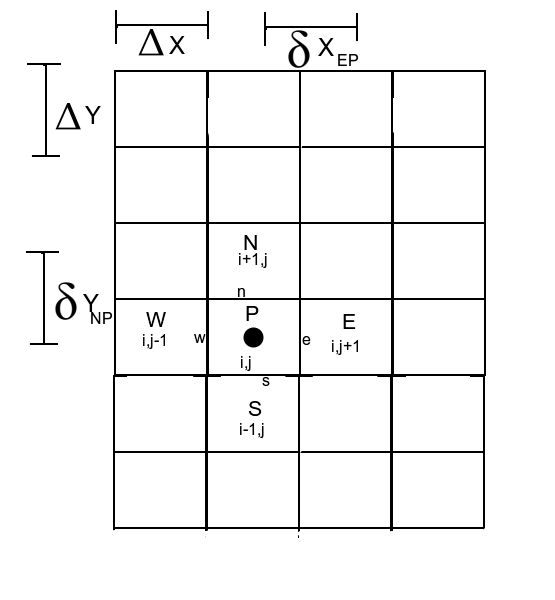
\includegraphics[width=\linewidth]{Stencil.png}
\caption{REPRESENTATION OF THE STENCIL FOR THE FINITE VOLUME APPROACH}
\label{fig:stencil}
\end{center}
\end{figure}

\begin{figure}[t]
\begin{center}
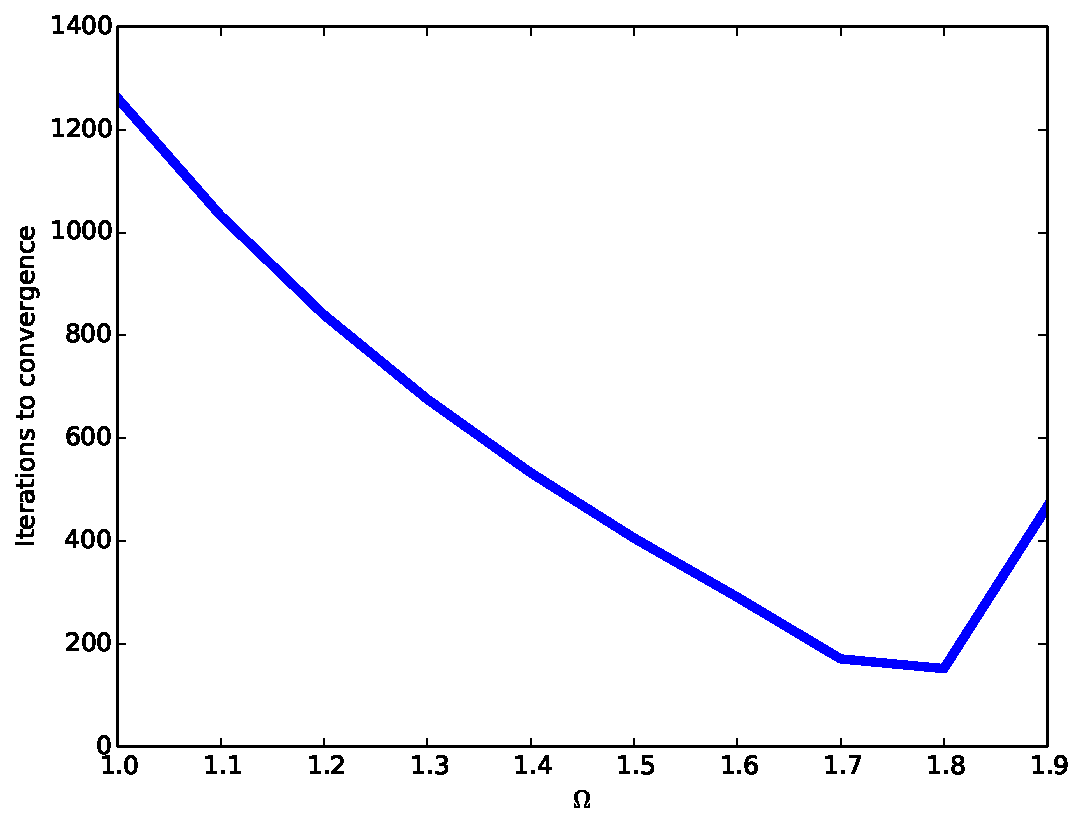
\includegraphics[width=\linewidth]{../Project1_code/Iterations.pdf}
\caption{PLOT SHOWING ITERATIONS TO NECESSARY CONVERGENCE FOR EACH VALUE OF $\Omega$ RELAXATION FACTOR}
\label{iterations}
\end{center}
\end{figure}

\begin{figure}[t]
\begin{center}
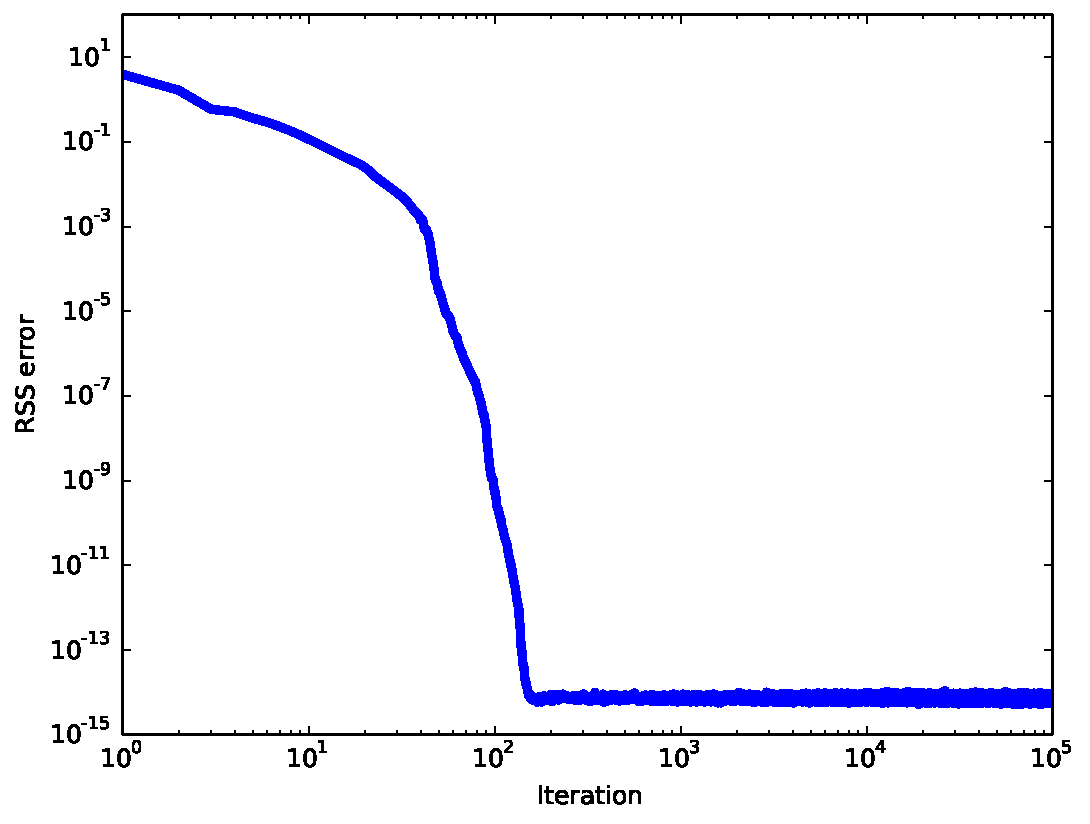
\includegraphics[width=\linewidth]{../Project1_code/convergence_long.pdf}
\caption{CONVERGENCE LOG-LOG PLOT OF THE ITERATION SOLUTION FOR MANY ITERATIONS}
\label{convergence}
\end{center}
\end{figure}

\begin{figure}[t]
\begin{center}
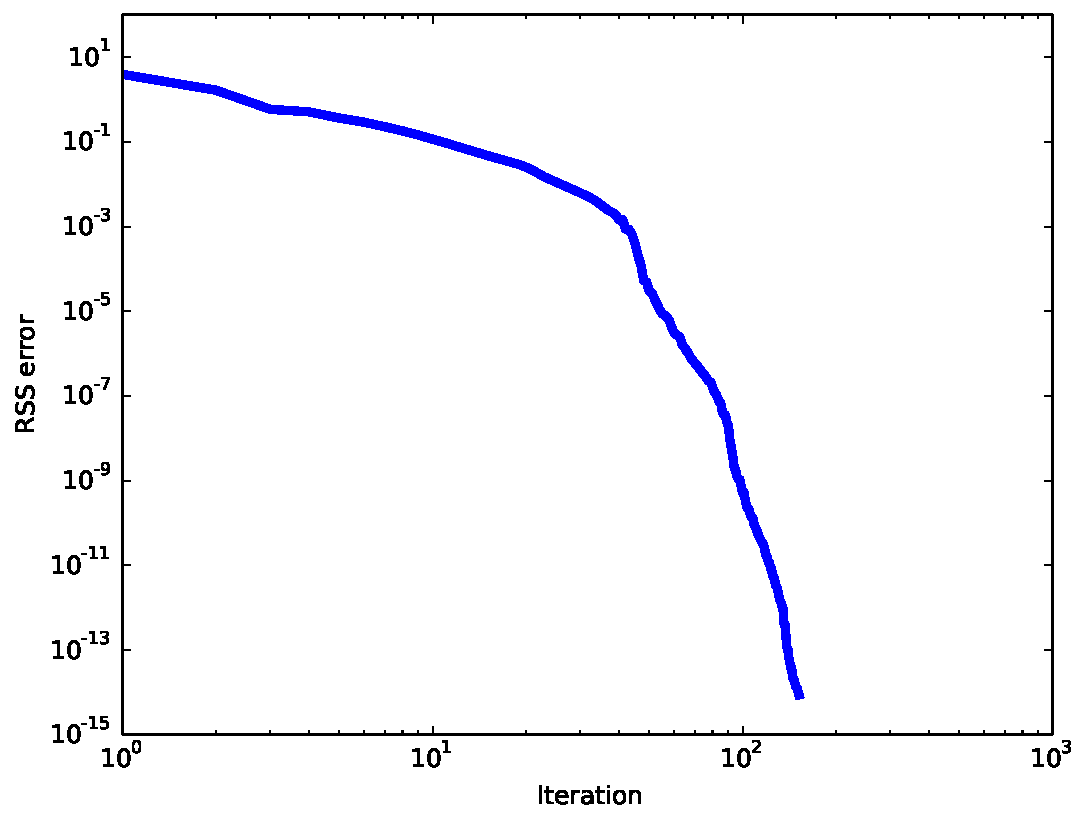
\includegraphics[width=\linewidth]{../Project1_code/convergence.pdf}
\caption{CONVERGENCE LOG-LOG PLOT OF THE ITERATION SOLUTION FOR 152 ITERATIONS}
\label{convergence2}
\end{center}
\end{figure}


\begin{figure}[t]
\begin{center}
    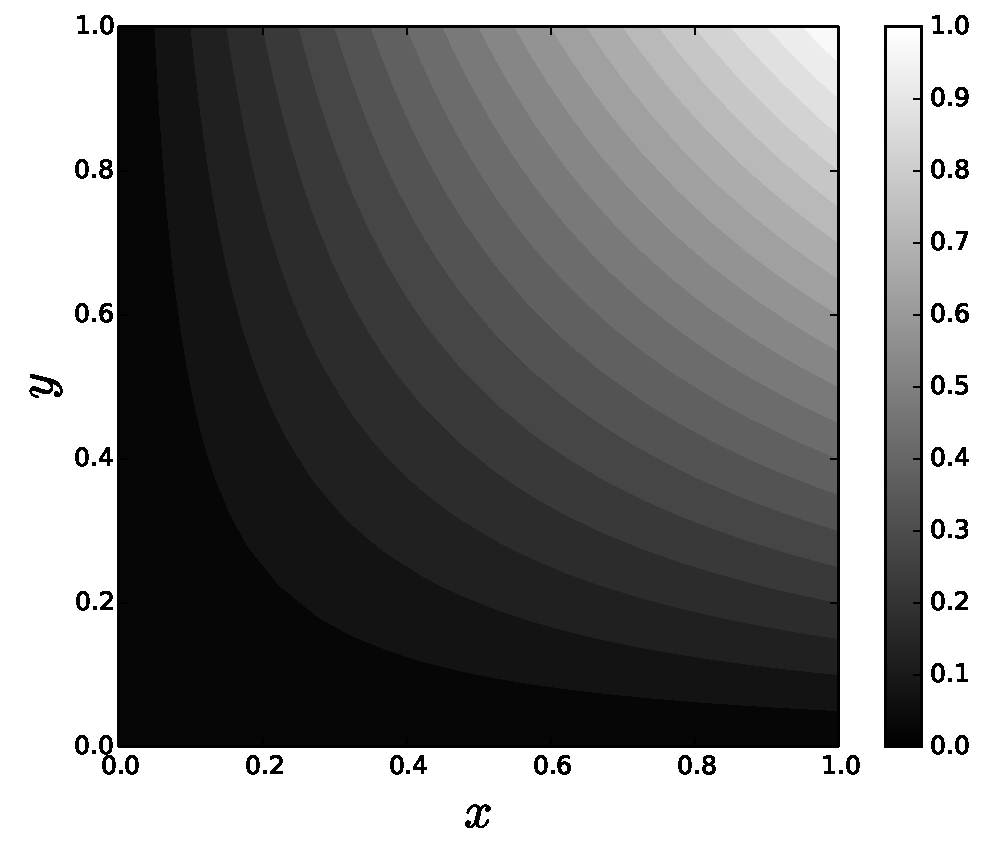
\includegraphics[width=\linewidth]{../Project1_code/phi.pdf}
    \caption{CONVERGED SOLUTION $\phi$ CONTOUR PLOT}
    \label{phi}
    \end{center}
\end{figure}

\begin{figure}[t]
\begin{center}
    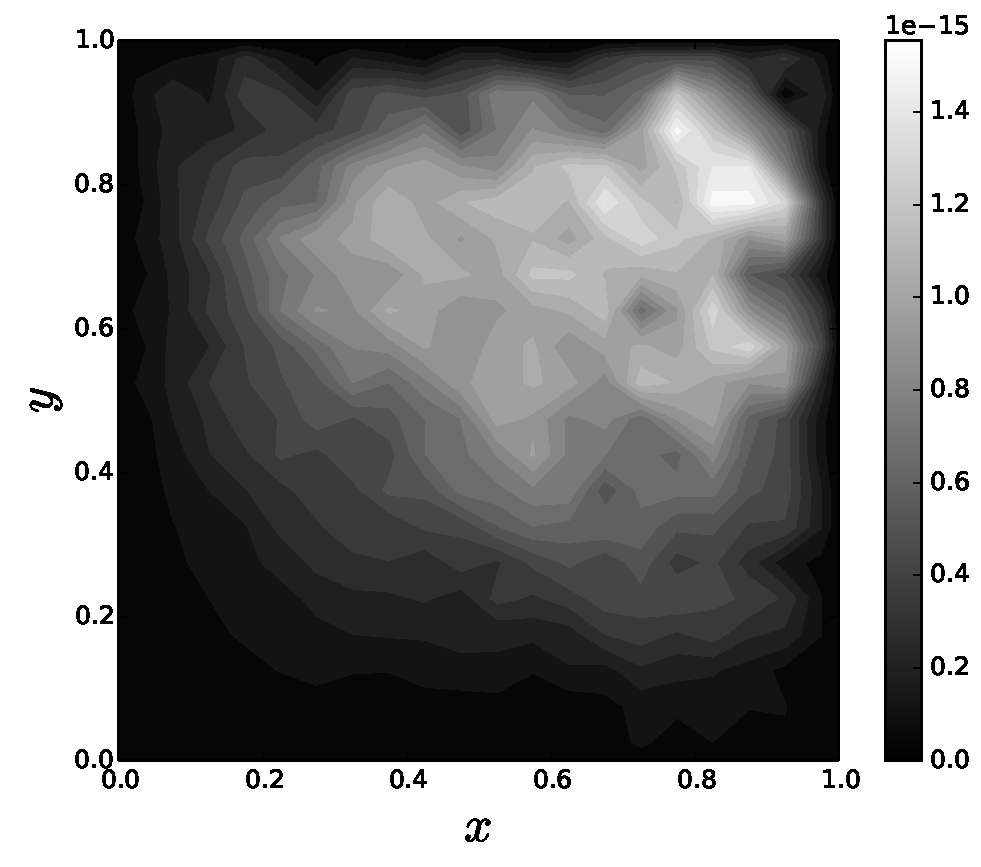
\includegraphics[width=\linewidth]{../Project1_code/error.pdf}
    \caption{CONTOUR PLOT SHOWING THE ERROR BETWEEN THE NUMERICAL AND ANALYTICAL SOLUTION}
    \label{error}
    \end{center}
\end{figure}

%%%%%%%%%%%%%%%%%%%%%%%%%%%%%%%%%%%%%%%%%%%%%%%%%%%%%%%%%%%%%%%%%%%%%%

\clearpage

\appendix

\section*{Appendix A: Code}

\lstinputlisting[language=Fortran]{../Project1_code/Project1.f90}



\end{document}
